\section{AMR-Based Detonation Solver in OpenFOAM}


\begin{frame}{Tested Solvers}
Solvers tested for their capability to model shocks and detonations:
\begin{itemize}
\item \textbf{rhoReactingFoam}: included with OpenFOAM, a density-based combustion solver
\item \textbf{rhoCentralFoam}: included with OpenFOAM and developed by Greenshields \textit{et. al.} \cite{greenshields}, a density-based solver that uses the central-upwind schemes of Kurganov and Tadmor \cite{kurganov1} 
\item \textbf{rhoReactingCentralFoam}: a solver combined by Caelan Lapointe with previous work done by Nakul \cite{nakul}, with AMR support
\end{itemize}
\end{frame}

\subsection{Governing Equations}

\begin{frame}[allowframebreaks]{Governing Equations}
Detonations were modeled using the reacting Navier-Stokes equations \cite{kuo,stokes}:
\begin{equation}
\frac{\partial \rho}{\partial t} + \nabla \cdot \left(\rho \bm{u}\right) = 0\,
\end{equation}
\begin{equation}
\frac{\partial \rho\bm{u}}{\partial t} + \nabla \cdot \left(\rho \bm{u}\otimes \bm{u}\right) + \nabla p -\mu\nabla^2\bm{u}= \bm{0}\,,
\end{equation}
\begin{equation}
\frac{\partial \rho E}{\partial t} + \nabla \cdot \left[\left(\rho E + p\right)\bm{u}\right] -\alpha\nabla^2 e = \dot{q}\,,
\end{equation}
\begin{equation}
\frac{\partial \rho Y_i}{\partial t} + \nabla \cdot \left(\rho Y_i \bm{u}\right) -\mu\nabla^2 Y_i= \dot{\omega}_i\,,
\end{equation}
where 
\begin{equation}
\dot{q} = \sum_{i = 1}^N \dot{\omega_i} \Delta h_{f,i}^0\,,
\end{equation}
%is the heat flux, $\dot{\omega}_i$ is the species source reaction rate, $\rho$ is the density, $\bm{u}$ is the fluid velocity vector, $Y_i$ is the mass fraction of the $i$th species, $E$ is the total energy, $p$ is the pressure, $\mu$ is the dynamic viscosity, $e$ is the internal energy, $\alpha$ is the thermal diffusivity and $\Delta h_{f,i}^0$ is the species formation enthalpy.
\end{frame}


\begin{frame}{Notes About Governing Equations}
\begin{itemize}
\item Specific heat $C_{p,i}=C_{p,i}(T)$ from NIST JANAF \cite{janaf} lookup tables.  
\item No explicit turbulence modeling, but turbulence can form
\begin{itemize}
    \item subgrid-scale turbulence structures averaged out numerically
    \item akin to implicit LES
\end{itemize}
\item Not modeling inviscid Euler equations; viscosity is accounted for with Sutherland \cite{sutherland} model:
\end{itemize}
\begin{equation}
\mu = \frac{A_s \sqrt{T_s}}{1 + \frac{T_s}{T}} \,,
\end{equation}
\end{frame}

\subsection{Chemistry Modeling}

\begin{frame}{Chemical Reactions}
Single-step stoichiometric hydrogen-air utilized for simplicity, which follows the following expression \cite{kuo}:
\begin{center}
\ch{2 H2 + 2 (O2 + 3.76 N2) -> 2 H2O + 7.52 N2}
\end{center}
with
\begin{table}[t!]
\centering
\begin{tabular}{cc}
Species & Mass Fraction \\ \hline
H\(_2\) & 0.02851 \\ 
H\(_2\)O & 0 \\
N\(_2\) & 0.745 \\ 
O\(_2\) & 0.226 \\ \hline
Total & 0.99951 \\ 
\end{tabular}
\end{table}
OpenFOAM allows for easy transitions between chemical models.
\end{frame}

\begin{frame}{Reaction Rate Modeling}
Arrhenius equation \cite{arrhenius} takes the form \cite{christ} 
\begin{equation}
\dot{\omega}_i = AT^\beta \exp\left(\frac{ -E_a}{R T}\right)\,,
\end{equation}
where $Ta = Ea/R$. Simulation values were explored, but we settled on 
\begin{equation}
   A = 1.4 \times 10^{13} ~ \text{m}^3\text{mol}^{-1}\text{s}^{-1},
   \qquad 
   Ta = 12996 ~\text{K},
   \qquad
   \beta = 0\,.
\end{equation}
with \(R = 368.9\) J/Kg-K. As shown later these reasonably match Chapman-Jouguet detonation theory \cite{chapman} along with other published values \cite{towery1,hashemi}.
\end{frame}

\subsection{Domain Setup}

\begin{frame}{Simulation Domain Setup}
Besides ignition region, domain is at 1 atm and 300 K
\begin{figure}[t!]
\centering
\includegraphics[width=0.8\textwidth]{../figs/domainBC.png}
%\caption{Geometry and domain setup with boundary conditions}
%\label{fig:domainBC}
\end{figure}%
\end{frame}

\subsection{Parallel Computing}

\begin{frame}{Parallel Computing: Decomposition}
%Domain is decomposed into chunks which are independently processed in parallel, communicating with MPI \cite{walker}. Decomposition defined in \texttt{decomposeParDict}. Several methods for decomposition:
%\begin{itemize}
%\item \texttt{simple}: define splits in each direction 
%\item \texttt{hierarchical}: \texttt{simple}, but with recursive ordering to splits
%\item \texttt{scotch}: minimizes boundaries between processors, can set weighting
%\item \texttt{manual}: manual cell allocation to each processor 
%\end{itemize}
%The \texttt{simple} method was used here. 
\begin{itemize}
\item Domain is decomposed into chunks which are independently processed in parallel, communicating with MPI \cite{walker}
\item Decomposition defined in \texttt{decomposeParDict}
\item Several methods for decomposing domain in OpenFOAM, but \texttt{simple} method was utilized which simply splits number of times in each direction
\end{itemize}
\end{frame}

\begin{frame}{Parallel Computing: Load Balancing}
\begin{figure}[p]
    \centering
    \begin{subfigure}[]{0.45\textwidth}
        \centering
        \includegraphics[width=0.9\textwidth]{../figs/parallel_short.png}
        \caption{Domain decomposed into typical chunks, bad for detonation and AMR load balancing}
        %\label{sfig:shortdecomp}
    \end{subfigure}%
    \begin{subfigure}[]{0.45\textwidth}
        \centering
        \includegraphics[width=0.9\textwidth]{../figs/parallel_long.png}
        \caption{Domain decomposed into long chunks, better for detonation and AMR load balancing}
        %\label{sfig:longdecomp}
    \end{subfigure}
    %\caption{Example domain decomposition techniques for parallel computing}
    %\label{fig:decomp}
\end{figure}%
\end{frame}

\subsection{Adaptive Mesh Refinement}

\begin{frame}{Adaptive Mesh Refinement: Splitting}
Adaptive meshing splits the cells using an octree splitting method:
\begin{figure}[]
\centering
\includegraphics[width=0.4\textwidth]{../figs/amr_example.png}
%\caption{Adaptive mesh refinement octree splitting method}
%\label{fig:octree}
\end{figure}%
This makes the AMR inherently three-dimensional. 
\end{frame}


\begin{frame}{Adaptive Mesh Refinement Parameters}
Allows for the mesh to refine and unrefine based on set parameters:
\begin{itemize}
\item \texttt{refineInterval}: frequency when active, based on time steps
\item \texttt{field}: which parameter to track
\item \texttt{lowerRefineLevel}: lower bound of active refinement 
\item \texttt{upperRefineLevel}: upper bound of active refinement
\item \texttt{unrefineLevel}: upper bound of unrefinement
%\item \texttt{nBufferLayers}: number of buffer cell layers between levels of refinement 
%\item \texttt{maxRefinement}: additional recursive refinement levels
\item \texttt{maxCells}: maximum cell count to trigger AMR update
\end{itemize}
\end{frame}

\begin{frame}{Adaptive Mesh Refinement: Refinement Levels}
\begin{columns}
\column{0.5\textwidth}
\texttt{maxRefinement}: Number of additional recursive refinement levels
\column{0.5\textwidth}
\begin{center}
\includegraphics[width=0.8\textwidth]{../figs/amr_refine.png}
\end{center}
\end{columns}
\end{frame}


\begin{frame}{Adaptive Mesh Refinement: Buffer Layers}
\begin{columns}
\column{0.5\textwidth}
\texttt{nBufferLayers}: Number of buffer cell layers between levels of refinement
\column{0.5\textwidth}
\begin{center}
\includegraphics[width=0.8\textwidth]{../figs/amr_buffer.png}
\end{center}
\end{columns}
\end{frame}


\begin{frame}{Adaptive Mesh Refinement: Detonation Wave}
\begin{figure}
\centering
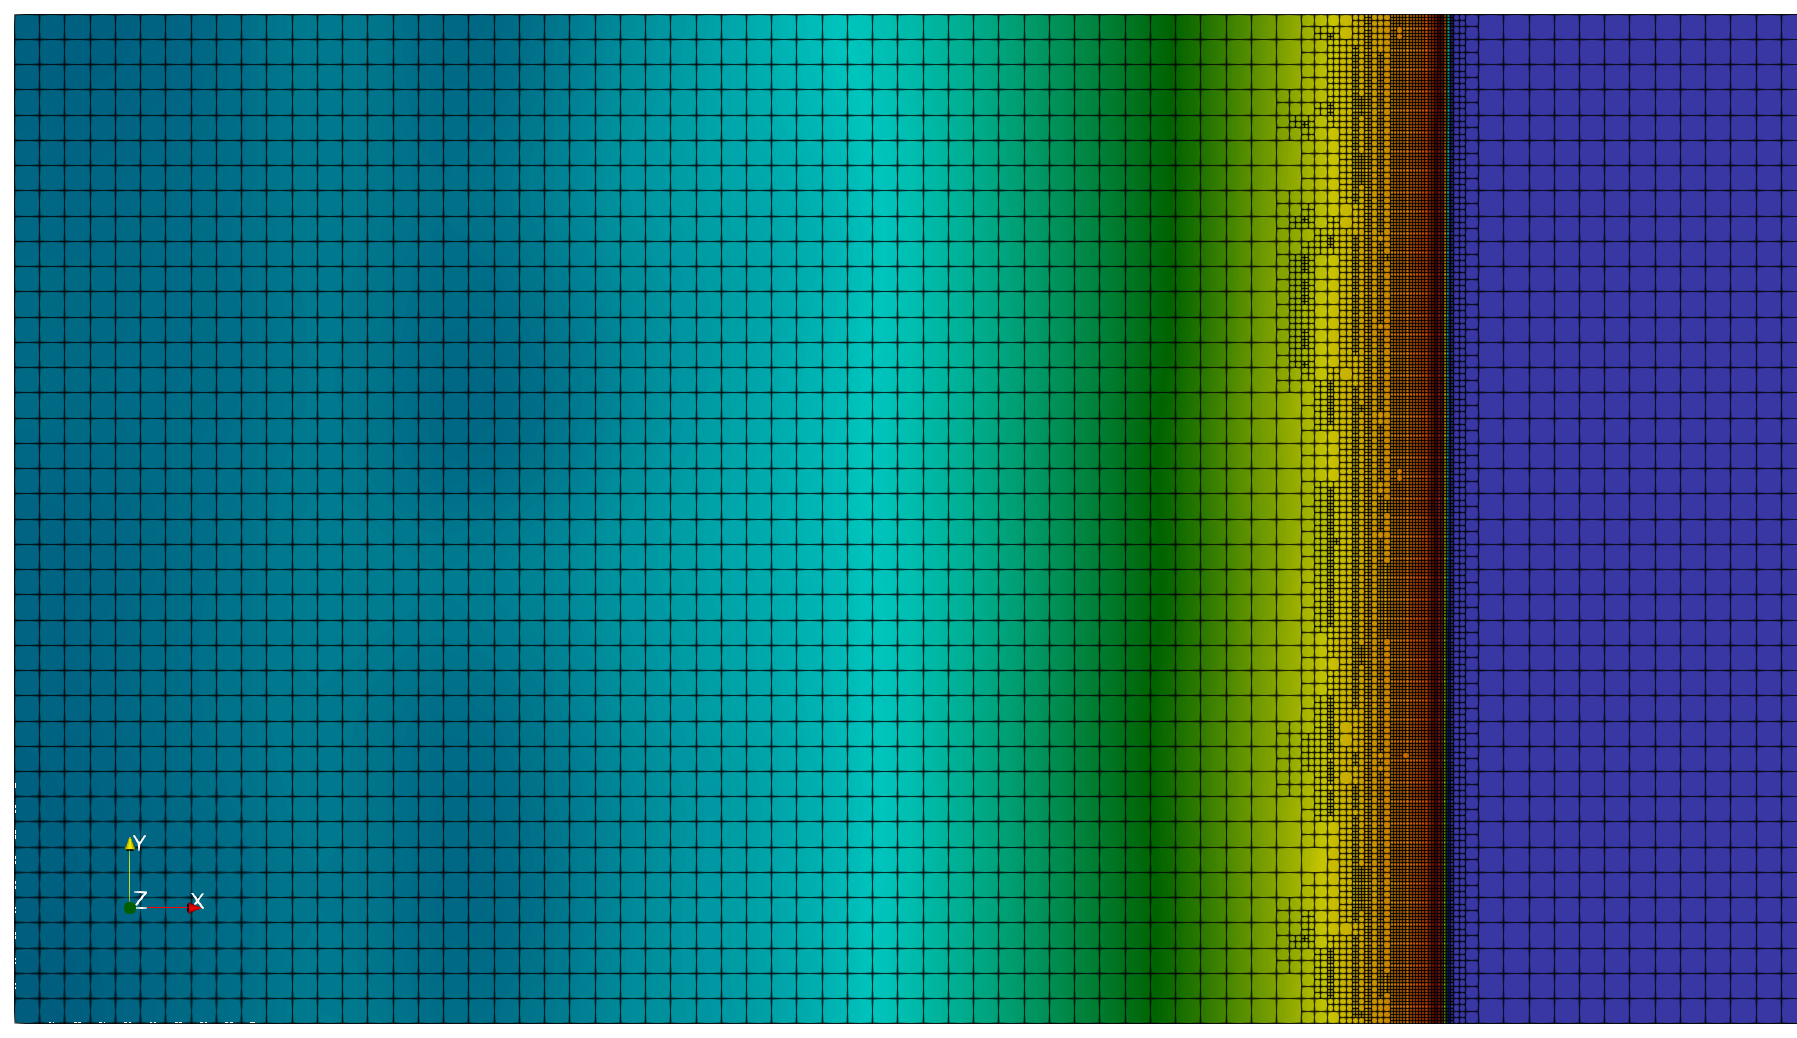
\includegraphics[width=0.7\textwidth]{../figs/amr_cells.png}
\caption{Three-level adaptive mesh refinement over a pressure field surface contour, with the detonation wave traveling from the -x wall to +x exit}
%\label{fig:examr}
\end{figure}
\end{frame}

\begin{frame}{Initial Meshing}
\begin{figure}[]
    \centering
    \begin{subfigure}[]{0.5\textwidth}
        \centering
        \includegraphics[width=\textwidth]{../figs/mesh/2Dmesh.png}
        \caption{Two-dimensional mesh}
    \end{subfigure}%
    \begin{subfigure}[]{0.5\textwidth}
        \centering
        \includegraphics[width=\textwidth]{../figs/mesh/3Dmesh.png}
        \caption{Three-dimensional mesh}
    \end{subfigure}
    %\caption{Static meshes used in OpenFOAM for detonation modeling, at an exaggerated unrefined resolution for example purposes}
    %\label{fig:meshcompare}
\end{figure}
\end{frame}

\subsection{Initial Work and Testing}

\begin{frame}{Initial Detonation Attempts}
First testing \texttt{rhoReactingFoam}, methane-oxygen without nitrogen was used, with corner ignition to test shock reflection and exit 
\begin{figure}[]
\centering
\includegraphics[width=0.9\textwidth]{../figs/cornerdet.png}
%\caption{Initial methane and oxygen detonation boundary condition test with corner detonation. Velocity magnitude is plotted here without scale to just check the solver and boundary conditions for modeling potential. Detonation was initiated in the lower left corner.}
%\label{fig:cornerdet}
\end{figure}%
Testing the detonation tube setup performed by Towery \textit{et. al.} \cite{towery1} was next, to be used as comparison. 
\end{frame}

\begin{frame}{\texttt{rhoReactingFoam} Problems}
\begin{columns}
\column{0.4\textwidth}
\begin{itemize}
\item Different static mesh resolutions were tested with \texttt{rhoReactingFoam}, but noise and instability in the solution was seen.
\item likely due to solver being more pressure-based than density-based
\end{itemize}
\column{0.6\textwidth}
\begin{figure}[]
\centering
\includegraphics[width=\textwidth]{../figs/rhoReactingFoam.png}
%\caption{Noise and instability in solution and shock capturing problems using the \texttt{rhoReactingFoam} solver}
%\label{fig:rrf}
\caption*{Pressure vs. Grid Location}
\end{figure}%
\end{columns}
\end{frame}

\begin{frame}{\texttt{rhoReactingCentralFoam} Selection and Validation}
\begin{columns}
\column{0.6\textwidth}
\begin{figure}[]
\centering
\includegraphics[width=\linewidth]{../figs/shocktube.png} 
%\caption{Shock tube validated test case included with OpenFOAM compared to hybrid solver}
%\label{fig:sod}
\end{figure}%

\column{0.4\textwidth}
\begin{itemize}
\item turned towards the solvers utilizing central-upwind schemes of Kurganov and Tadmor \cite{kurganov1}
\item used the shock tube test to validate shock-capturing capability
\end{itemize}
\end{columns}
\end{frame}
